\documentclass[11pt, a4paper]{article}

% --- Tegnsett, språk og typografi ---
\usepackage[utf8]{inputenc}
\usepackage[T1]{fontenc}
\usepackage[norsk]{babel}
\usepackage{lmodern}
\usepackage{microtype}

% --- Sideoppsett og marger ---
\usepackage[a4paper, top=2.5cm, bottom=2.5cm, left=2.5cm, right=2.5cm]{geometry}
\usepackage{setspace}
\setstretch{1.12}

% --- Grafikk, farger og tabeller ---
\usepackage{graphicx}
\usepackage[dvipsnames]{xcolor}
\usepackage{booktabs}
\usepackage{tabularx}
\usepackage{multirow}
\usepackage{caption}
\usepackage{subcaption}
\usepackage{enumitem}

% --- Matematikk og tekniske enheter ---
\usepackage{amsmath, amssymb}
\usepackage{siunitx}
\sisetup{
    output-decimal-marker = {,},
    exponent-product = \cdot,
    group-separator = {\,}
}

% --- Bokser og fremheving ---
\usepackage[most]{tcolorbox}

% --- Fargedefinisjoner ---
\definecolor{navyblue}{RGB}{11, 60, 93}
\definecolor{accentblue}{RGB}{0, 102, 204}
\definecolor{darkgray}{RGB}{60, 64, 67}
\definecolor{lightgray}{RGB}{245, 247, 250}
\definecolor{boxbg}{RGB}{248, 250, 252}

% --- Topp- og bunntekst ---
\usepackage{fancyhdr}
\pagestyle{fancy}
\fancyhf{}
\fancyhead[L]{\small\textsf{\color{darkgray}Kongsberg Your Extreme 2026 \textbar\ Oppgave 1: «Når vi må bruke det vi har»}}
\fancyhead[R]{\small\textsf{\color{navyblue}\textbf{Prosjekt Meierikjeden}}}
\fancyfoot[C]{\small\textsf{\color{darkgray}Side \thepage}}
\renewcommand{\headrulewidth}{0.4pt}
\renewcommand{\footrulewidth}{0pt}

% --- Overskriftstyling ---
\usepackage{titlesec}
\titleformat{\section}
  {\color{navyblue}\normalfont\Large\bfseries\sffamily}
  {\thesection}{1em}{}
\titleformat{\subsection}
  {\color{navyblue}\normalfont\large\bfseries\sffamily}
  {\thesubsection}{1em}{}
\titleformat{\subsubsection}
  {\color{navyblue}\normalfont\normalsize\bfseries\sffamily}
  {\thesubsubsection}{1em}{}

% --- Bildetekster ---
\captionsetup{
    font=small,
    labelfont={bf, color=navyblue},
    labelsep=period,
    margin=1cm
}

% --- Hyperlenker ---
\usepackage{hyperref}
\hypersetup{
    colorlinks=true,
    linkcolor=navyblue,
    citecolor=accentblue,
    urlcolor=accentblue,
    pdfauthor={Your Extreme Gruppe},
    pdftitle={Prosjekt Meierikjeden - Your Extreme 2026},
    pdfsubject={Sivil beredskap og gjenbruk av næringsmiddelinfrastruktur}
}

% =========================================================================
% DOKUMENTSTART
% =========================================================================
\begin{document}

% --- FORSIDE ---
\begin{titlepage}
    \centering
    \vspace*{0.5cm}
    
    {\small\textsf{\textbf{\color{navyblue}KONGSBERG GRUPPEN \textbar\ CASEKONKURRANSE YOUR EXTREME 2026}}\par}
    {\small\textsf{\color{darkgray}Oppgave 1: «Når vi må bruke det vi har»}\par}
    
    \vspace{2.0cm}
    \hrule height 2pt
    \vspace{0.6cm}
    
    {\Huge\bfseries\sffamily\color{navyblue} Prosjekt Meierikjeden \par}
    \vspace{0.4cm}
    {\Large\sffamily Mobil og steril drikkevannsforsyning gjennom sivil næringsmiddelinfrastruktur \par}
    
    \vspace{0.6cm}
    \hrule height 0.8pt
    \vspace{1.5cm}
    
    {\large\textsf{\textbf{Gjenbruk av automatiserte CIP-anlegg og melketankbilflåten som nasjonal beredskapsforsyning ved akutt biologisk vannforurensning}}\par}
    
    \vfill
    
    \begin{tcolorbox}[colback=lightgray, colframe=navyblue, width=0.9\textwidth, arc=2mm]
    \centering
    \small\sffamily
    \textbf{Faglig profil og kjernekonsept:}\\
    Maskinteknisk innovasjon (\textit{AquaFeed Manifold}) kombinert med næringsmiddelteknologi (CIP), mikrobiologisk/allergen-barrierestyring og dynamisk to-faset flåtelogistikk innenfor rammen av det norske Totalforsvaret.
    \end{tcolorbox}
    
    \vspace{1.5cm}
    
    \begin{minipage}{0.48\textwidth}
        \flushleft
        \small\textsf{\textbf{Innlevert av:}}\\
        \textsf{Prosjektgruppe Meierikjeden}\\
        \textsf{Your Extreme 2026}
    \end{minipage}
    \hfill
    \begin{minipage}{0.48\textwidth}
        \flushright
        \small\textsf{\textbf{Dato:}}\\
        \textsf{Høst 2026}\\
        \textsf{Kongsberg, Norge}
    \end{minipage}

    \vspace{0.5cm}
\end{titlepage}

% --- INNHOLD OG MODULÆRE SEKSJONER ---
\pagenumbering{arabic}
\setcounter{page}{1}

\section*{Sammendrag (Executive Summary)}
\addcontentsline{toc}{section}{Sammendrag}

Når flom eller sabotasje fører til kloakkoverløp i en bys råvannskilder, kollapser tradisjonell beredskap på få timer: Flaskevannlogistikken kveles av emballasje og dødvolum, kommunale spylebiler er ubrukelige grunnet biofilm og kjemikalierester, mens generelle kokeanbefalinger lammer drift ved sykehus og sykehjem.

\textbf{Prosjekt Meierikjeden} løser denne sårbarheten gjennom sivil gjenbruk (\textit{repurposing}) av Norges mest finmaskede, lukkede transportnettverk: meieriindustrien. Ved å mobilisere eksisterende melketankbiler i elektropolert syrefast stål (\textsc{aisi} 316L) og sterilisere dem via automatiserte, lukkede \textsc{cip}-stasjoner (\textit{Cleaning-In-Place} med lut-, syre- og dampsterilisering ved \SI{85}{\celsius}), etableres en steril forsyningslinje fra fire uavhengige reservekilder.

Konseptets mekaniske kjerneinnovasjon er \textbf{«AquaFeed Manifold»}---en prefabrikkert tapperigg med tilbakeslagsventiler som monteres verktøyløst på bilenes utløp på under to minutter. Gjennom en flåte på 15 biler distribueres \SI{900000}{\liter} sterilt drikkevann per døgn. Dette dekker basalbehovet til \num{300000} innbyggere og sikrer full drift ved akuttmottak og dialyseenheter, uten milliardinvesteringer i ny infrastruktur.

\begin{tcolorbox}[colback=boxbg, colframe=navyblue, arc=2mm, title=\textbf{Hovedtall og nøkkeldata}, fonttitle=\bfseries\sffamily]
\begin{itemize}[leftmargin=1.5em, itemsep=0.1em]
    \item \textbf{Døgnkapasitet:} \SI{900000}{\liter} sterilt vann per døgn (15 biler à \SI{20}{\cubic\meter}, 3 rotasjoner/døgn).
    \item \textbf{Befolkningsdekning:} \num{300000} personer ved \SI{3}{\liter}/døgn (eller \num{75000} innbyggere med \SI{12}{\liter}/døgn).
    \item \textbf{Mekanisk innovasjon:} \textit{AquaFeed Manifold} i \textsc{aisi} 316L (\SI{20000}{NOK}/stk; \SI{1}{MNOK} for 50 enheter).
    \item \textbf{Allergensikkerhet:} Kjemisk hydrolyse og to-trinns verifisering (\textsc{atp} + lateral-flow, $< \SI{1}{ppm}$).
    \item \textbf{Totalforsvar:} To-faset flåtestyring som verner dyrevelferd og avverger melkedumping.
\end{itemize}
\end{tcolorbox}

\newpage

\section{Krisescenario og svikt i dagens beredskap}
\label{sec:scenariet}

\subsection{Det akutte forurensningsscenariet}
Norsk drikkevannsforsyning er basert på sårbare overflatekilder. Scenarioet tar utgangspunkt i en norsk by med \num{50000} til \num{100000} innbyggere som rammes av et intensivt flomforløp etter ekstremnedbør. Flomvannet overbelaster fellesavløpsnettet, hvorpå tilbakeslag og oversvømte pumpestasjoner medfører massivt urenset kloakkoverløp i byens primære råvannskilde og sentrale høydebasseng.

Vannet kontamineres akutt med patogene mikroorganismer, primært \textit{Campylobacter jejuni}, enteropatogene \textit{Escherichia coli} og norovirus. Før rutineanalyser rekker å stanse distribusjonen, har smittestoffene spredt seg i rørnettet. Kommuneoverlegen beordrer umiddelbar stenging av nettet for konsum ledsaget av kokevarsel. Byen står overfor en akutt helse- og forsyningskrise.

\subsection{Hvorfor etablert beredskap svikter}
Når ledningsnettet settes ut av spill, kollapser tradisjonelle krisetiltak i løpet av timer:
\begin{enumerate}[leftmargin=1.5em, itemsep=0.2em]
    \item \textbf{Flaskevann-kollaps:} Dagligvarehandelen opererer med slanke «just-in-time»-lagre, og butikkhyller tømmes innen tre timer. Palltransport av flaskevann er logistisk ineffektivt grunnet emballasjevekt og dødvolum; å dekke dagsbehovet til \num{75000} innbyggere krever over 20 semitrailere daglig, med uoverkommelige trafikkpropper som resultat.
    \item \textbf{Institusjonell lammelse:} Kokevarsel fungerer for friske husholdninger, men lammer helseinstitusjoner. Akuttsykehus, sykehjem og dialyseenheter krever titusenvis av liter sterilt vann daglig til pasientbehandling, sårstell, dialyse, hygiene og matproduksjon. Helseforetakene mangler kjelekapasitet og personell til storskala koking og nedkjøling.
    \item \textbf{Forurenset kommunalt materiell:} Brann- og spylebiler kan ikke benyttes til drikkevann. Tanker og slanger inneholder rust, etablert biofilm samt giftige rester av kjemikalier og \textsc{pfas}-holdig slukkeskum som ikke lar seg dekontaminere i felten.
    \item \textbf{Mangel på bulkbeholdere:} Kommuner disponerer knapt sertifiserte næringsmiddeltanker for bulktransport. Innleie tar dager, mens behovet for rent vann er akutt.
\end{enumerate}

Dermed oppstår et livstruende kapasitetsgap: Byen trenger storskala distribusjon av sterilt drikkevann, men mangler mobile, godkjente beholdere. Som vist i figur~\ref{fig:kart} etablerer Prosjekt Meierikjeden en mobil forsyningskjede over vei som bypasser det forurensede rørnettet.

\begin{figure}[htbp]
    \centering
    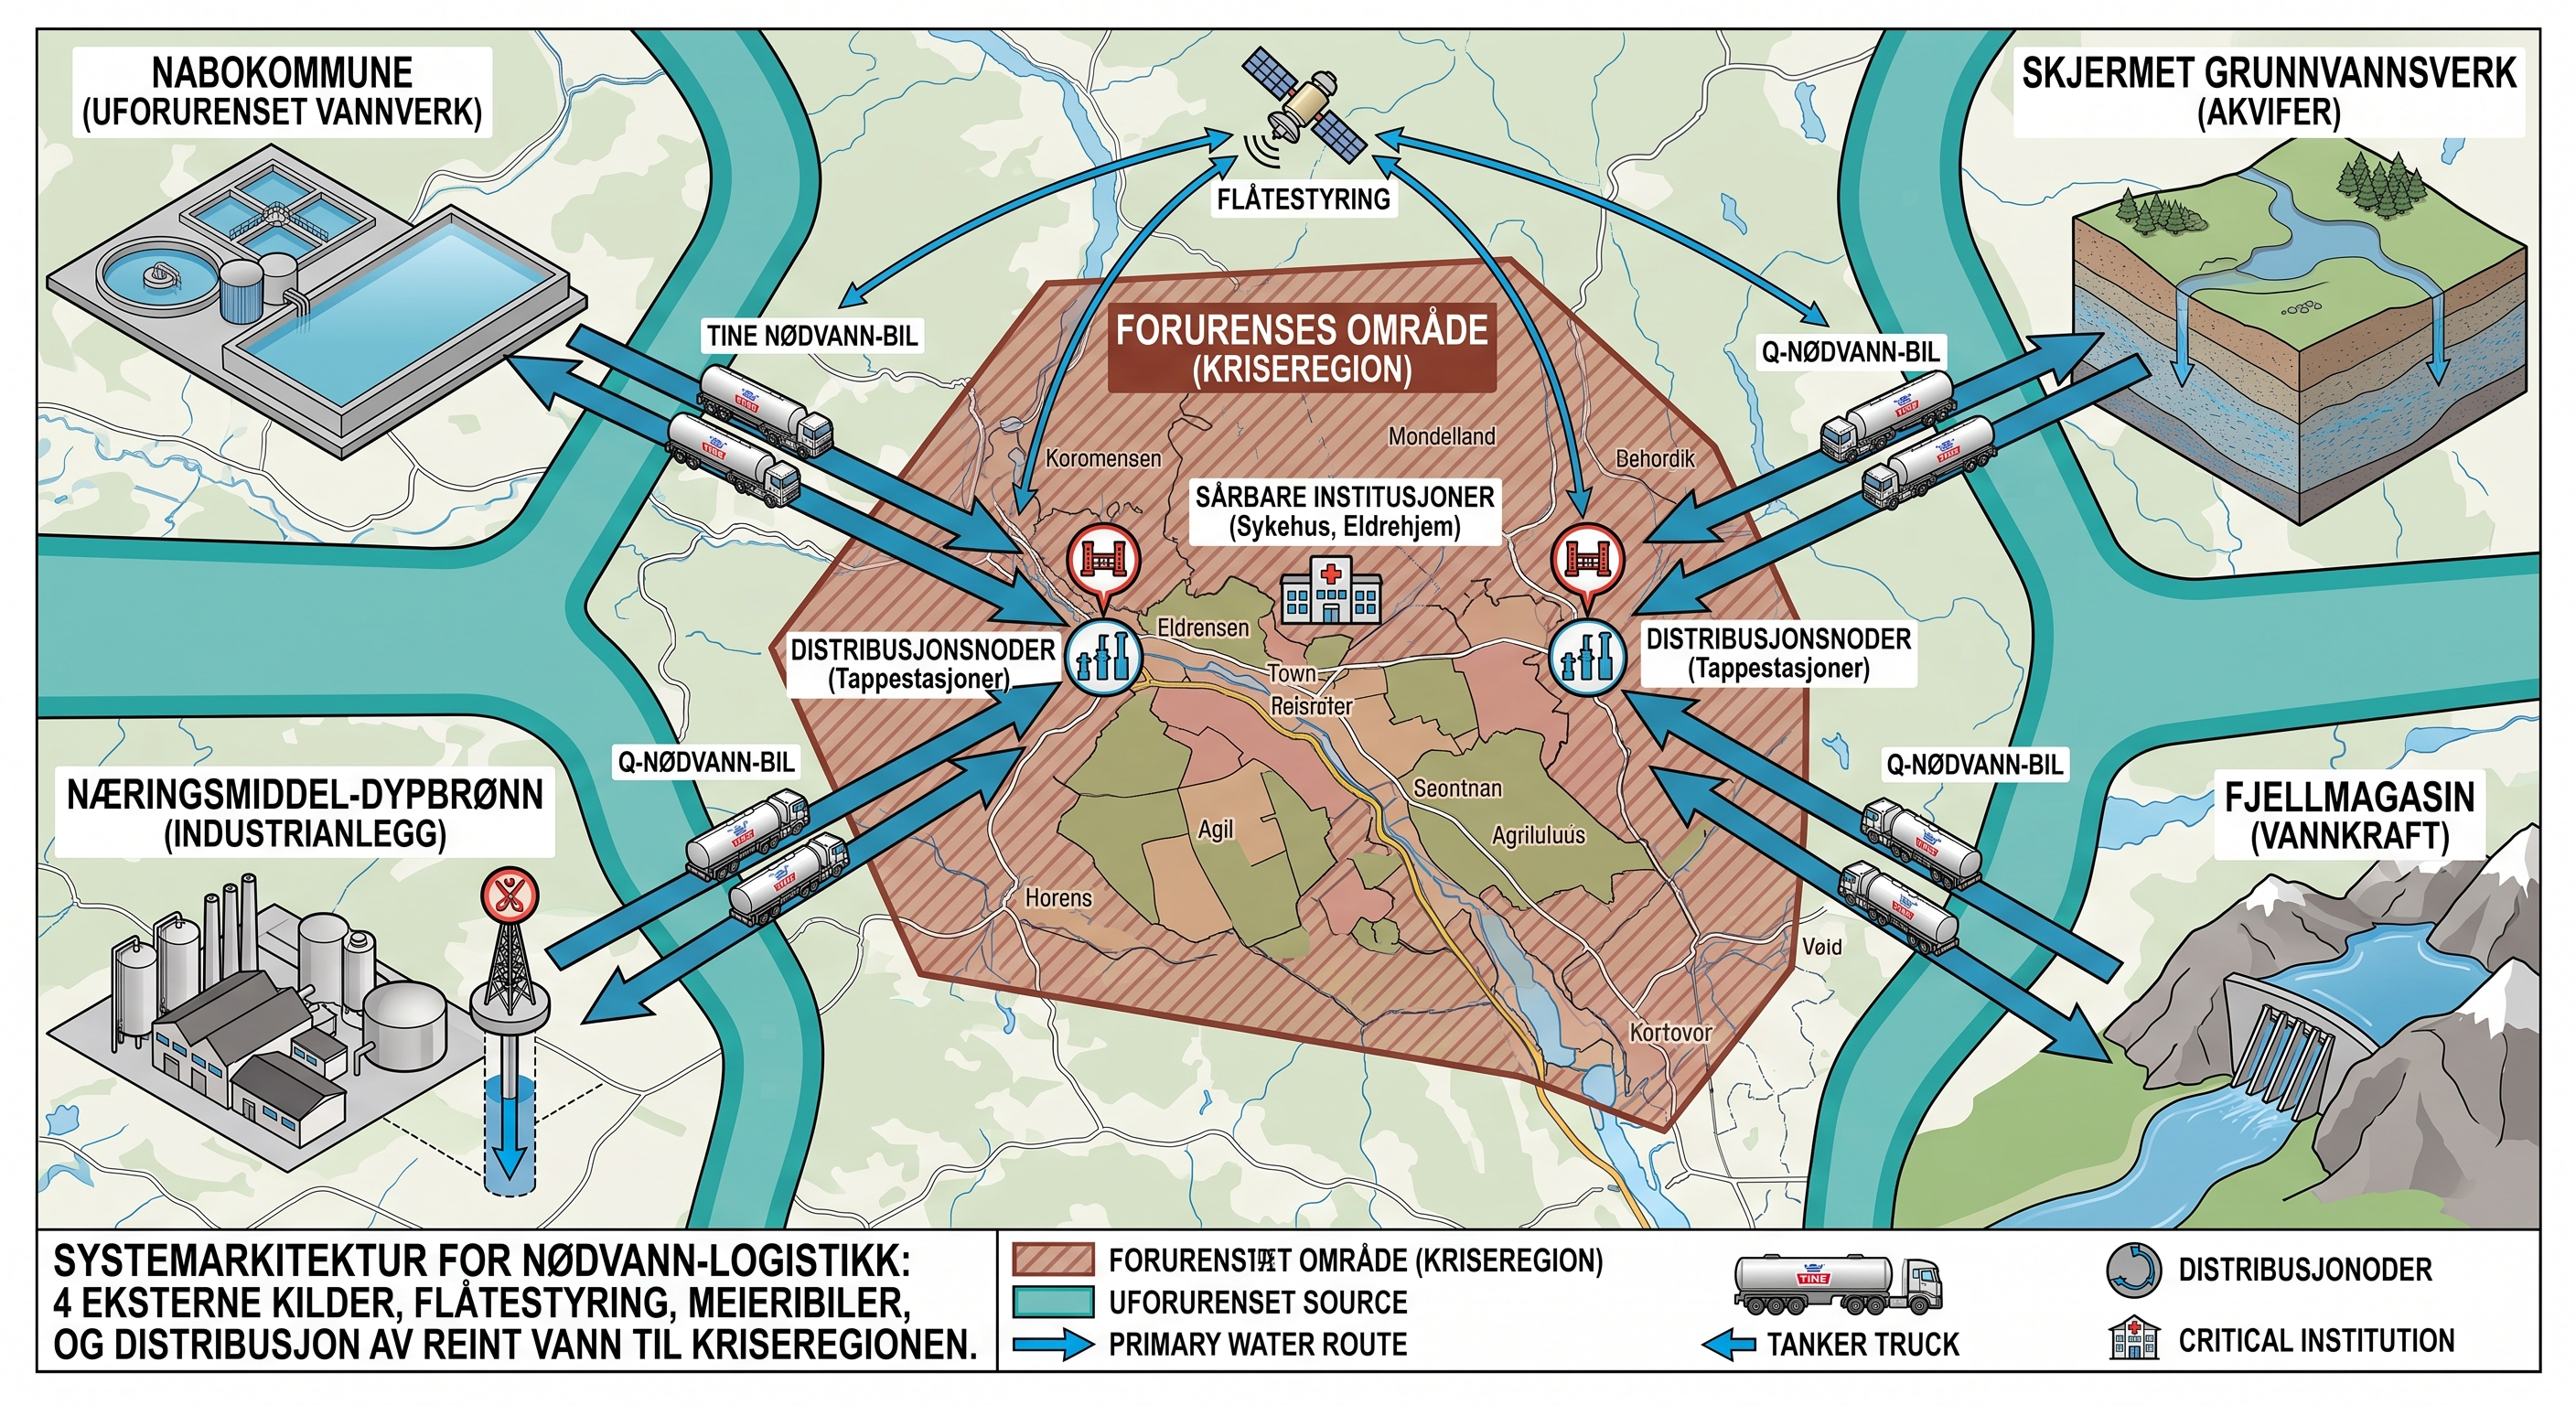
\includegraphics[width=0.95\textwidth]{Figures/Kart_over_forskyningskjede.jpg}
    \caption{Systemarkitektur for Prosjekt Meierikjeden: Mobilisering av meieriflåten etablerer en «virtuell rørledning» over vei fra fire uavhengige reservekilder, med to-spors forsyning til sykehus (Linje A) og sivile utdelingspunkter (Linje B).}
    \label{fig:kart}
\end{figure}


\section{Kjerneteknologi: Sivil næringsmiddelinfrastruktur}
\label{sec:kjerneteknologi}

Å frakte drikkevann til sårbare grupper og sykehus under en biologisk krise stiller strengere hygienekrav enn ordinære kommunale vannrør. Norsk meieriindustri transporterer daglig råmelk---en biologisk væske med ideelle vekstvilkår for patogener. Teknologien som sikrer råmelkens mikrobiologiske kvalitet utgjør en sovende beredskapsressurs.

\subsection{Materialteknologi og biofilmfrie overflater}
Konstruksjonen av melketankbiler skiller seg radikalt fra ordinære industritankbiler:
\begin{itemize}[leftmargin=1.5em, itemsep=0.2em]
    \item \textbf{Elektropolert syrefast stål:} Tanker og røropplegg er produsert i austenittisk rustfritt stål (\textsc{aisi} 316L / \textsc{en} 1.4404) med molybdenlegering, elektropolert til $Ra \le \SI{0.4}{\micro\meter}$. Den mikroskopiske planheten eliminerer sprekker der mikroorganismer kan hefte, hvilket gjør biofilmdannelse fysisk umulig.
    \item \textbf{Fullisolert termoskonstruksjon:} Dobbelveggede tanker isolert med høydensitets polyuretanskum (\textsc{pur}) sikrer at forhåndskjølt vann holder en stabil temperatur under \SI{6}{\celsius} gjennom transporten, selv på varme sommerdager, og hindrer bakteriell vekst.
\end{itemize}

\subsection{Autonom termisk og kjemisk sterilisering (\textsc{cip})}
Før innsats steriliseres tankbilene ved meierienes helautomatiserte og lukkede \textsc{cip}-stasjoner (\textit{Cleaning-In-Place}), som illustrert i figur~\ref{fig:cip}:
\begin{enumerate}[leftmargin=1.5em, itemsep=0.15em]
    \item \textbf{Forhåndsspyling:} Lunkent vann (\SI{45}{\celsius}) fjerner grove væskerester.
    \item \textbf{Alkalisk fase (lutvask):} \SI{2.0}{\percent} natriumhydroksid (\textsc{naoh}) ved \SI{75}{\celsius} i 10 minutter forsåper fett og hydrolyserer proteinbindinger.
    \item \textbf{Mellomspyling:} Rentvannsskylling fjerner kjemikalierester.
    \item \textbf{Syrefase:} \SI{1.5}{\percent} salpetersyre (\textsc{hno}$_3$) ved \SI{65}{\celsius} nøytraliserer baserester og løser opp mineraler og melkestein.
    \item \textbf{Termisk sterilisering:} Avsluttende overopphetet vann og damp ved $\ge \SI{85}{\celsius}$ i 15 minutter.
\end{enumerate}

Prosessen overvåkes kontinuerlig av sensorer for ledningsevne, turbiditet og temperatur. Digital vaskelogg verifiserer $\log 6$-reduksjon (\num{99.9999}\% reduksjon) av patogener.

\begin{figure}[htbp]
    \centering
    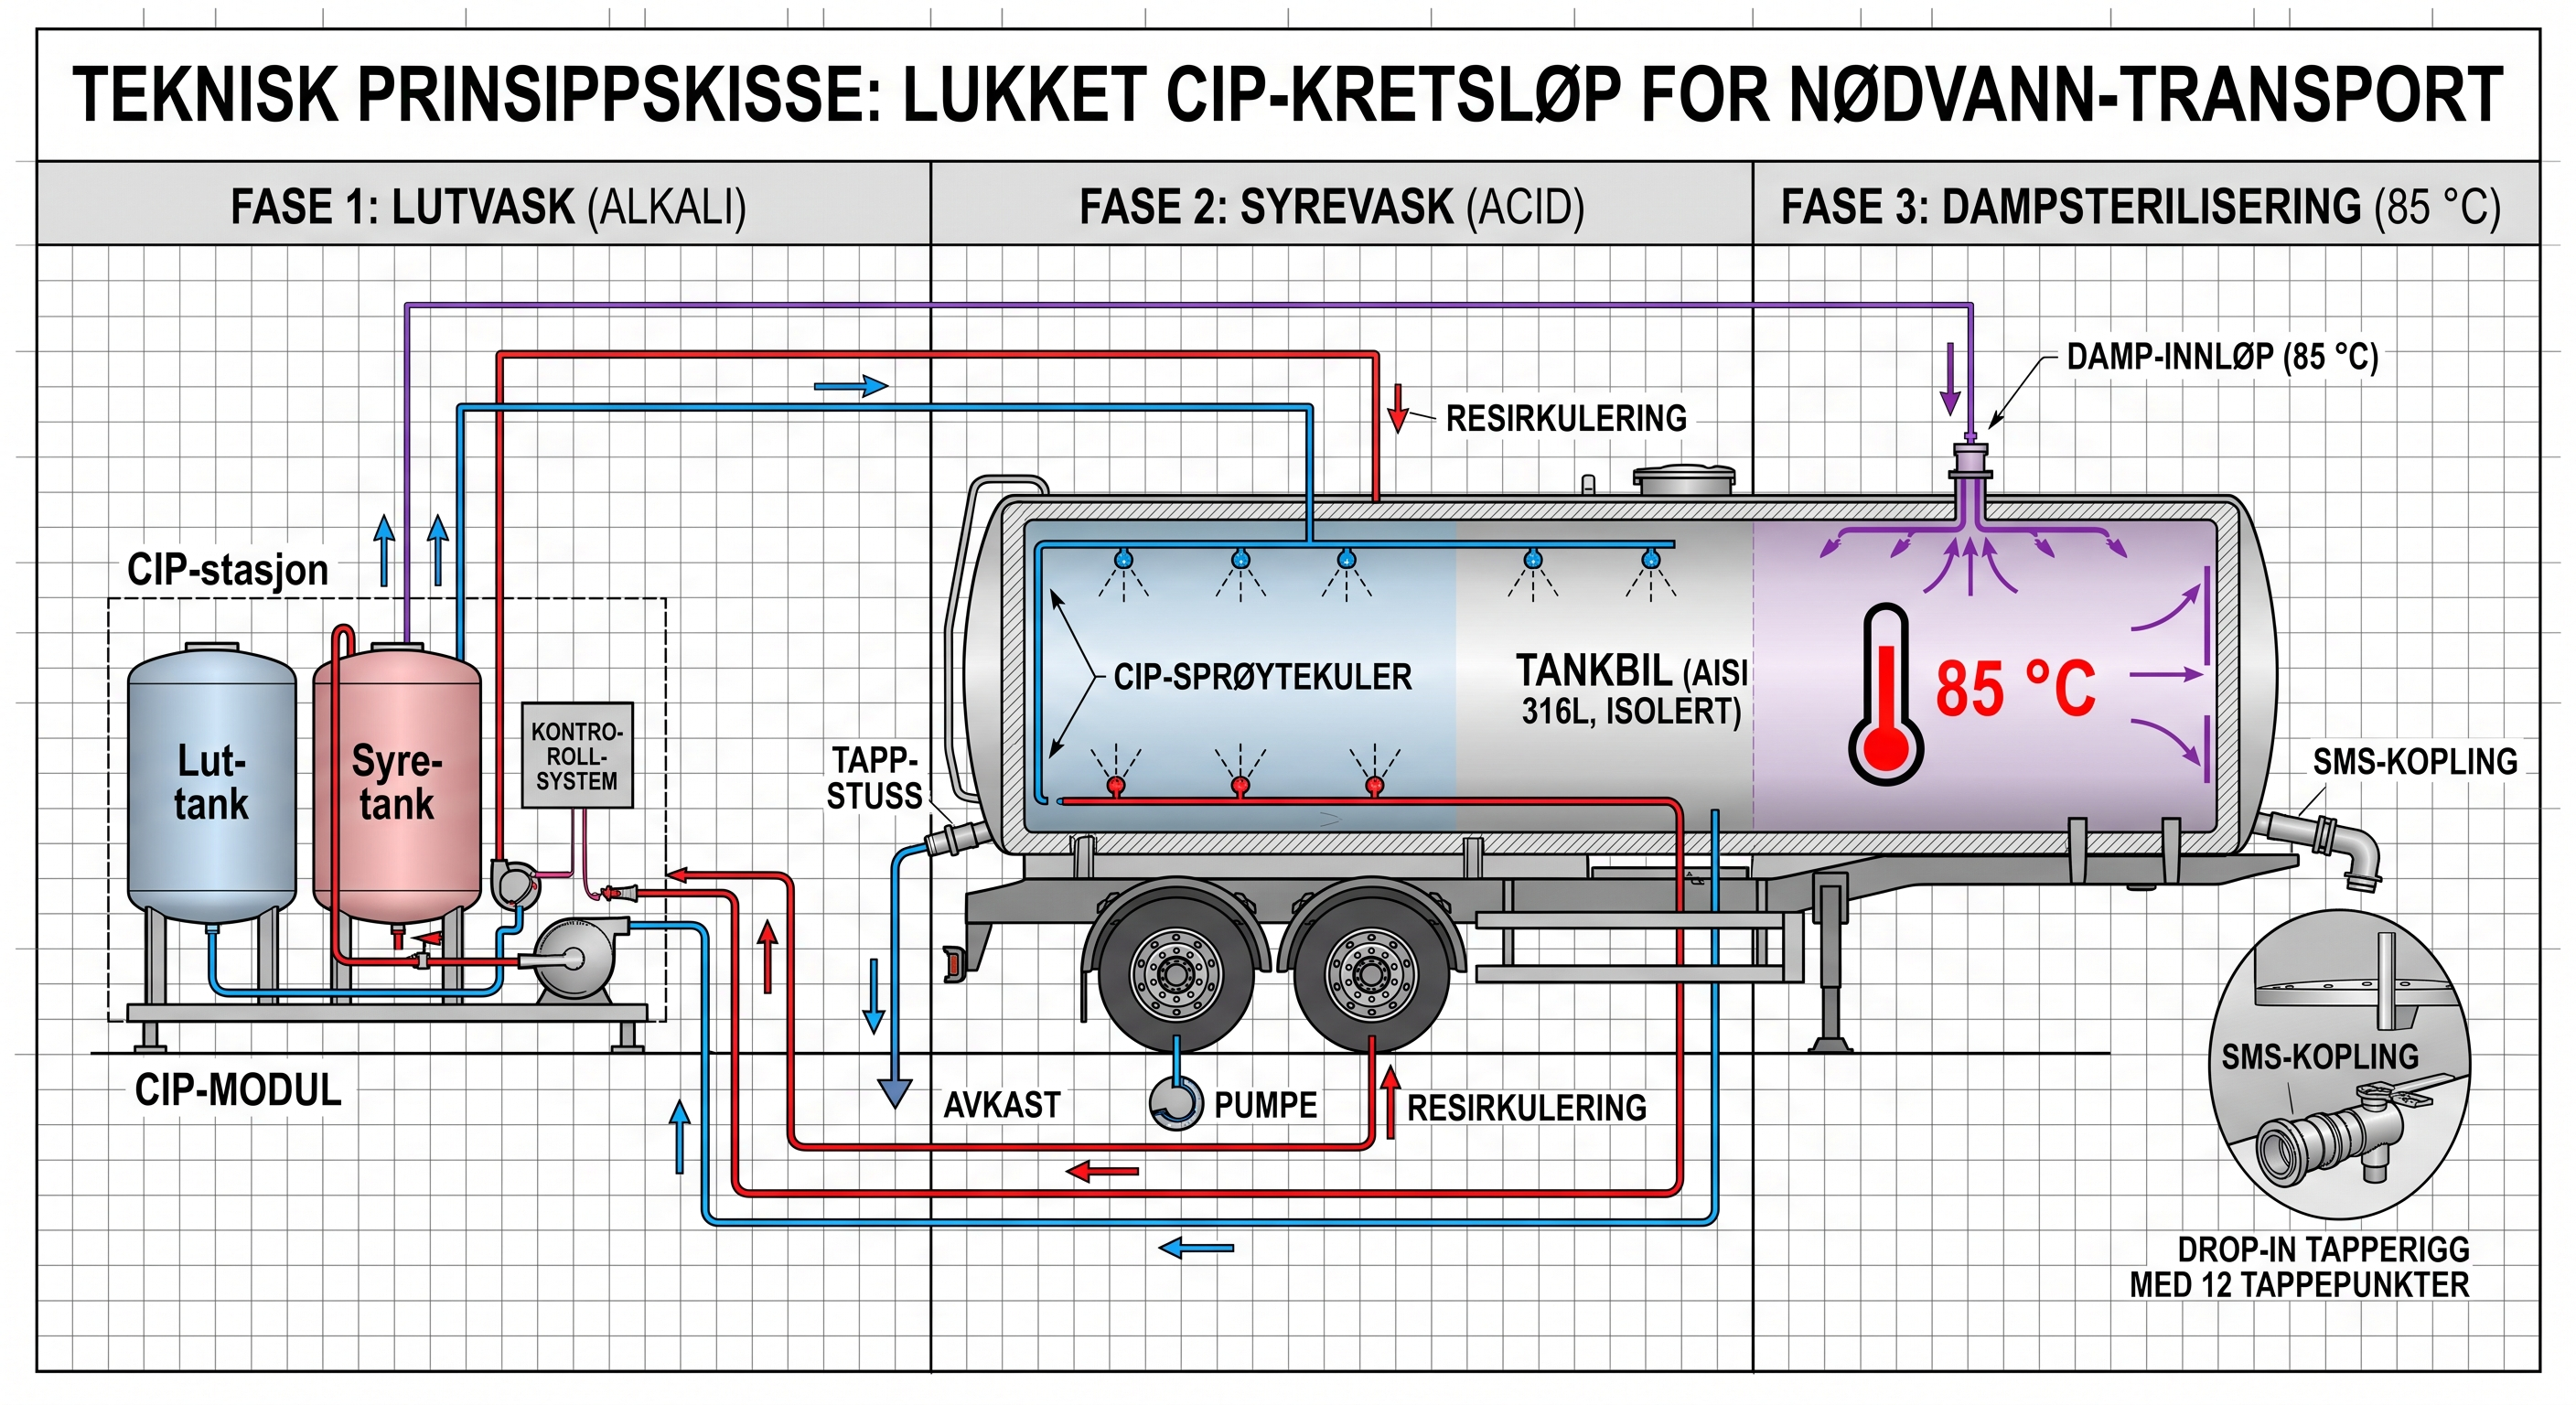
\includegraphics[width=0.92\textwidth]{Figures/CIP-process.jpg}
    \caption{Skjematisk oversikt over den automatiserte \textsc{cip}-vaskesyklusen. Vekslingen mellom termisk energi, lut og syre garanterer kjemisk renhet og bakteriologisk sterilitet.}
    \label{fig:cip}
\end{figure}

\subsection{Håndtering av melkeproteiner og allergenbarrierer}
Alvorlig melkeallergi mot kasein eller myseprotein ($\beta$-laktoglobulin) kan utløse anafylaksi hos spedbarn og pasienter. Prosjekt Meierikjeden etablerer derfor en uavhengig allergenbarriere basert på kjemisk degradering og to-trinns feltverifisering:
\begin{enumerate}[leftmargin=1.5em, itemsep=0.15em]
    \item \textbf{Alkalisk hydrolyse:} Varm lutvask (\SI{2.0}{\percent} \textsc{naoh}, \SI{75}{\celsius}, $\text{pH} > 12.5$) spalter melkeproteinenes peptidbindinger irreversibelt og denaturerer de immunogene epitopene.
    \item \textbf{To-trinns feltverifisering før fylling:}
    \begin{itemize}[leftmargin=1.5em, itemsep=0.1em]
        \item \textit{\textsc{atp}-bioluminescens:} Svaberprøve analyseres på 30 sekunder; måleverdier under 10 \textsc{rlu} bekrefter fravær av organisk restmateriale.
        \item \textit{Lateral-flow hurtigteststrips:} Immunokromatografiske strips dyppes i skyllevannet. Deteksjonsgrensen på $< \SI{1}{ppm}$ (\SI{1}{\micro\gram\per\milli\liter}) gir visuelt svar innen 5 minutter.
    \end{itemize}
\end{enumerate}
Vann fylles først når begge tester er negative, hvilket garanterer null allergirisiko.

\subsection{Hydraulisk kapasitet og lukkede kretsløp}
Hver tankbil rommer \num{15000} til \SI{25000}{\liter} og disponerer sanitære impellerpumper i syrefast stål (\SI{1000}--\SI{1500}{\liter\per\minute}). En tank på \SI{20}{\cubic\meter} fylles eller tømmes dermed på under 20 minutter. Utlufting skjer gjennom sterile \textsc{hepa}-luftfiltre for å hindre luftbåren kontaminering.


\section{Det tekniske bindeleddet: «AquaFeed Manifold»}
\label{sec:innovasjonen}

En melketankbil er konstruert for rørtransport mellom gård og meieri, ikke for manuell utlevering til allmennheten. For å transformere en melkebil til et operativt distribusjonspunkt på under fem minutter, har gruppen utviklet det mekaniske bindeleddet \textbf{«AquaFeed Manifold»} (figur~\ref{fig:tapperigg}). Dette utgjør prosjektets sentrale mekaniske innovasjon.

\begin{figure}[htbp]
    \centering
    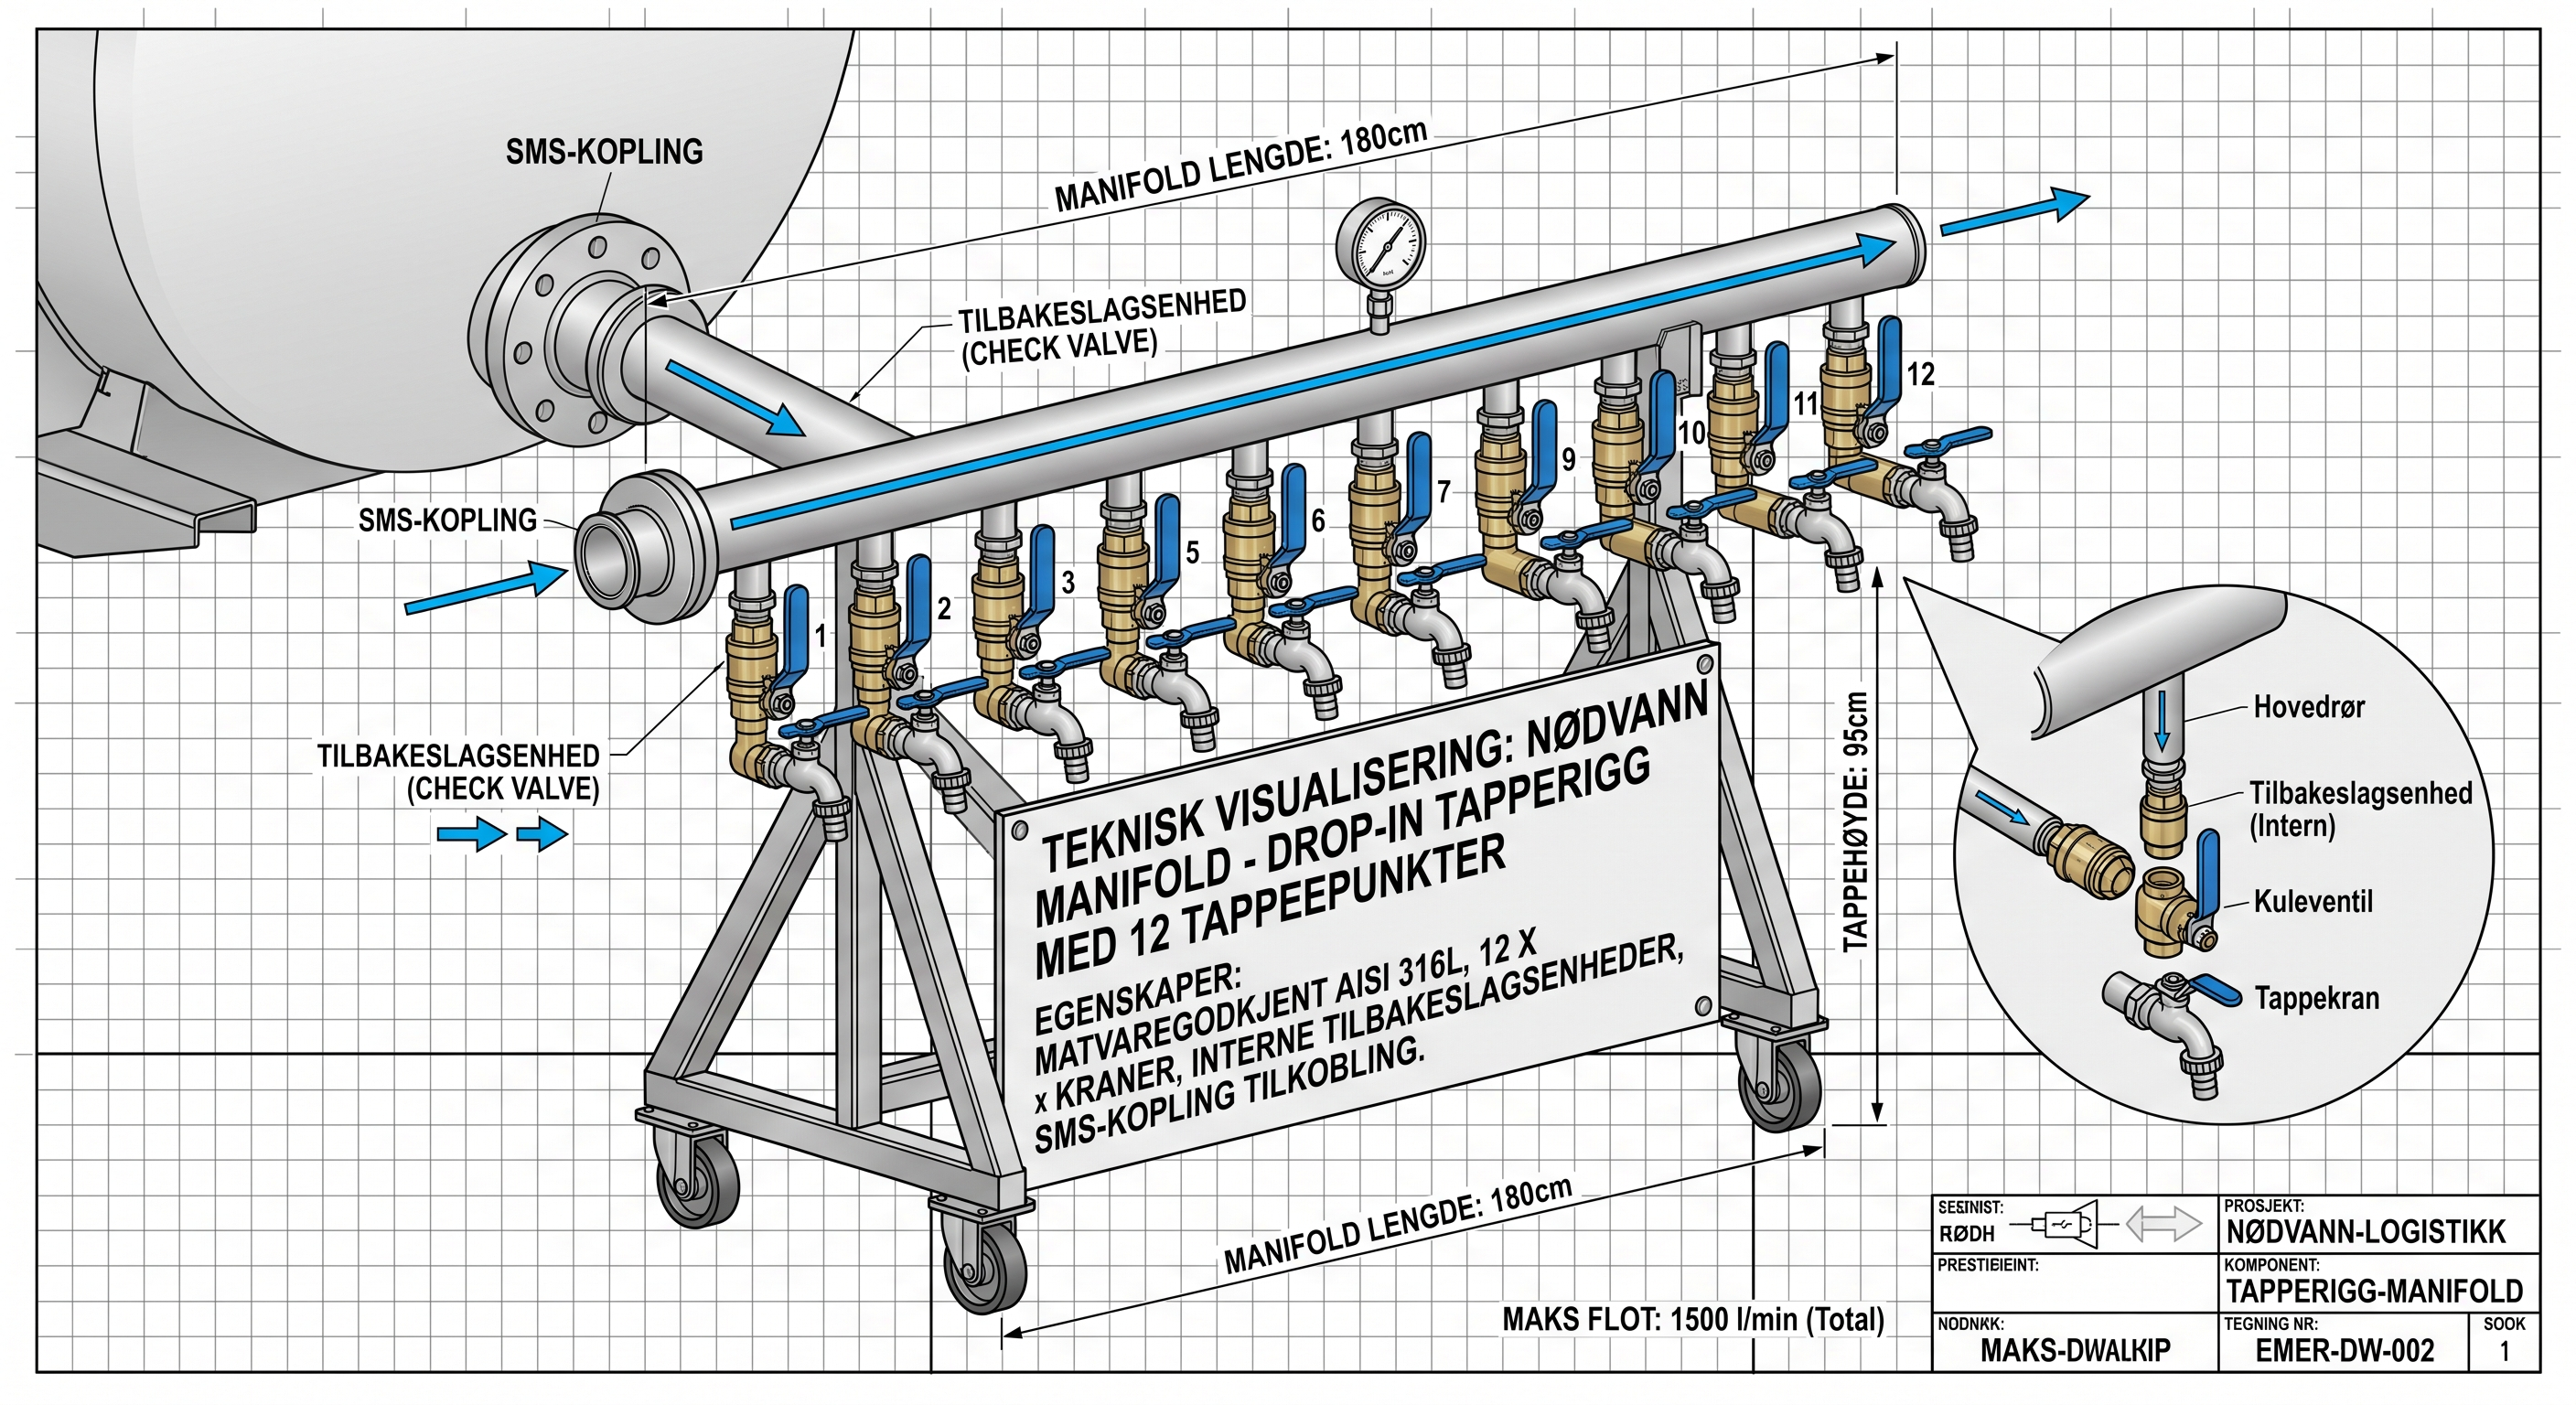
\includegraphics[width=0.92\textwidth]{Figures/Tapperigg.jpg}
    \caption{Den egenutviklede «AquaFeed Manifold»-tapperiggen montert på melkebilens bakre utløp. Modulær oppbygging med 10 parallelle tappepunkter, tilbakeslagsventiler, integrert trykkreduksjon og sammenleggbar støtteramme.}
    \label{fig:tapperigg}
\end{figure}

\subsection{Mekanisk konstruksjon og grensesnitt}
Norske melkebiler benytter sanitære koblinger iht. \textsc{sms} 1145 eller \textsc{din} 11851. Riggen fabrikkeres i elektropolert syrefast stål (\textsc{aisi} 316L):
\begin{itemize}[leftmargin=1.5em, itemsep=0.2em]
    \item \textbf{Verktøyløs hurtigkobling:} Riggen festes direkte til bilens \textsc{dn}65/\textsc{dn}76 bunnutløp via en standard \textsc{sms}-mutter med \textsc{epdm}-pakning. Montasjen utføres av sjåføren på under to minutter.
    \item \textbf{Ergonomisk støtteramme:} En integrert, sammenleggbar ramme i rørstål felles ut ved ankomst, avlaster utløpsventilen og plasserer kranene i arbeidshøyde (\SI{90}{\centi\meter}). Under transport lagres den i bilens sideskap.
\end{itemize}

\subsection{Beskyttelse mot krysskontaminering og tilbakesug}
For å eliminere smittefare fra befolkningens kanner har manifolden tre fysiske barrierer:
\begin{enumerate}[leftmargin=1.5em, itemsep=0.15em]
    \item \textbf{Fjærbelastede tilbakeslagsventiler:} Hver av de 10 tappekranene har en tilbakeslagsventil (\textit{non-return}) som stenger momentant ved trykkfall, slik at tilbakesug inn i tanken er fysisk umulig.
    \item \textbf{Berøringsfri geometri:} Tappedysene er skråstilt \ang{45} nedover med fri høyde over dryppristen, hvilket forhindrer kontakt med medbrakte kanner.
    \item \textbf{Flow- og trykkontroll:} En integrert membranventil regulerer trykket til et laminært arbeidstrykk på \num{1.5}--\SI{2.0}{\bar}. En 10-liters beholder fylles på 15--20 sekunder uten sprut.
\end{enumerate}

\subsection{Vinterdrift og universelt adaptersett}
For å sikre drift ved minusgrader er manifolden utstyrt med en integrert \SI{24}{\volt} selvbegrensende varmekabel (\SI{150}{\watt}) koblet til bilens strømuttak, samt hurtigtømmende bunnkraner for sekundrask drenering.

For oppkobling mot eksterne vannkilder medfølger et adaptersett i syrefast stål:
\begin{itemize}[leftmargin=1.5em, itemsep=0.2em]
    \item Overganger fra \textsc{sms}/\textsc{din} til brannvesenets Nor-lås type 1/2 og Storz B/C.
    \item Integrert \SI{100}{\micro\meter} partikkelfilter som fanger opp rust og sedimenter før tanken fylles.
\end{itemize}

\subsection{«Den siste meteren»: Sivil forurensningsbarriere}
Sterilt tankvann forringes dersom befolkningen tapper på urene bøtter. «Den siste meteren» sikres gjennom to tiltak:
\begin{itemize}[leftmargin=1.5em, itemsep=0.2em]
    \item \textbf{Sterile foldekanistere:} Sivilforsvaret og Røde Kors deler ut forhåndslagret, sammenleggbare 10-liters næringsmiddelgodkjente foldekanistere (\textsc{bpa}-frie).
    \item \textbf{Desinfeksjonssluse:} Innbyggere passerer en sluse med håndsprit og overflatedesinfeksjon for kanner før tapping.
\end{itemize}

\subsection{Kostnadskalkyle og nasjonal beredskapsreserve}
Riggen krever ingen elektronisk styring og kan serieproduseres rimelig:
\begin{itemize}[leftmargin=1.5em, itemsep=0.2em]
    \item \textbf{Enhetskostnad:} Fabrikasjon i syrefast stål (\textsc{aisi} 316L) inkludert ventiler, adaptersett og varmekabel er kalkulert til \num{15000}--\SI{25000}{NOK} per enhet.
    \item \textbf{Nasjonal reserve:} En reserve på 50 rigger koster ca. \SI{1.0}{MNOK}. Ved å forhåndslagre rigger ved landets 15 største meierier sikres nasjonal dekning med responstid under to timer.
\end{itemize}


\section{Kildestrategi og ruteplanlegging}
\label{sec:kildestrategi}

Når byens primærvannverk og rørnett er slått ut, er melkeflåtens styrke dens geografiske mobilitet. I stedet for å rense lokalt flomvann, oppretter prosjektet en «virtuell rørledning» over vei fra fire uavhengige reservekilder utenfor det rammede nedbørsfeltet.

\subsection{De fire uavhengige reservevannkildene}
\begin{enumerate}[leftmargin=1.5em, itemsep=0.25em]
    \item \textbf{Næringsmiddelindustriens dypbrønner og prosessanlegg:}
    Regionale meierier, bryggerier og slakterier disponerer egne dype grunnvannsbrønner og industrielle renseanlegg med flertrinns barrierer (ultrafiltrering, omvendt osmose og \textsc{uv}-bestråling). 
    \textit{Logistisk gevinst:} Tankbilen steriliseres i meieriets \textsc{cip}-anlegg, rygger 30 meter til fabrikkens interne rentvannsuttak, fylles i lukket sløyfe og sendes direkte ut.
    \item \textbf{Uberørte nabovannverk (Interkommunal veiforbindelse):}
    Nabokommunen 30--50 km unna henter vann fra et adskilt, uforurenset nedbørsfelt. Mange kommuner mangler fysiske overføringsrør grunnet topografi. Melkebilene fungerer som en fleksibel bypass: De kobler seg til nabovannverkets hydranter via adaptersettet og frakter vannet over kommunegrensen.
    \item \textbf{Skjermede grunnvannsbrønner i dype løsmasser:}
    Akviferer i dype sand- og gruslag påvirkes ikke av overflateflom og kloakkoverløp. Tykke sedimentlag danner et naturlig geologisk filter som sikrer mikrobiologisk trygt vann. Bilene kobles direkte til pumpehusenes ventiler.
    \item \textbf{Vannkraftmagasiner og alpine inntak:}
    Flomforurensningen skjer i lavlandet der avløp flyter over. I alpine inntaksdammer oppstrøms for bosetning finnes store mengder uberørt smelte- og regnvann. Bilene kan fylles direkte fra kraftverkenes driftsvannveier eller tømmeventiler.
\end{enumerate}

\subsection{Aksellast, flominfrastruktur og \textsc{vts}-integrasjon}
En fullastet tre- eller fireakslet melkebil har en totalvekt på 32 til 50 tonn. Under flom trues veiinfrastrukturen av erosjon og svekkede broer:
\begin{itemize}[leftmargin=1.5em, itemsep=0.2em]
    \item \textbf{Sanntidskobling mot Vegtrafikksentralen (\textsc{vts}):} Flåtestyringen integreres mot Statens vegvesens \textsc{vts}-database over stengte veier. Navigasjonssystemet ruter bilene utelukkende langs verifiserte \textsc{bk}10-korridorer (10 tonns aksellast / 50--60 tonns totalvekt).
    \item \textbf{Sikkerhetskorridorer:} Transporten ledes over høyereliggende europaveier og fylkesveier utenom flomutsatte stikkrenner. Ved usikker bæreevne på sekundære broer benyttes toakslede biler (\SI{15}{\cubic\meter}) for redusert marktrykk.
\end{itemize}


\section{Dimensjonering, logistikk og operasjonsmodell}
\label{sec:dimensjonering}

Beregningene under demonstrerer at en beskjeden andel av meieriflåten har tilstrekkelig hydraulisk og logistisk kapasitet til å dekke en hel regions vannbehov.

\subsection{Matematisk omløpsmodell}
Modellen bygger på empiriske driftsparametere fra norsk tankbiltransport:
\begin{itemize}[leftmargin=1.5em, itemsep=0.15em]
    \item Tankvolum ($V$): \SI{20}{\cubic\meter} (\SI{20000}{\liter}).
    \item Avstand ($d$): \SI{30}{\kilo\meter} én vei (\SI{60}{\kilo\meter} tur/retur kilde).
    \item Gjennomsnittsfart ($v$): \SI{50}{\kilo\meter\per\hour} (inkludert flomomkjøringer).
\end{itemize}

Total syklustid per rotasjon ($T_{\text{rot}}$) defineres ved:
\begin{equation}
    T_{\text{rot}} = t_{\text{fyll}} + t_{\text{transitt}} + t_{\text{loss}} + t_{\text{buffer}}
    \label{eq:syklus}
\end{equation}
hvor leddene kvantifiseres som følger:
\begin{align*}
    t_{\text{fyll}} &= \frac{V}{Q_{\text{pumpe}}} = \frac{\SI{20000}{\liter}}{\SI{1200}{\liter\per\minute}} \approx \SI{17}{\minute}, \\
    t_{\text{transitt}} &= \frac{2d}{v} = \frac{\SI{60}{\kilo\meter}}{\SI{50}{\kilo\meter\per\hour}} = \SI{1.2}{\hour} = \SI{72}{\minute}, \\
    t_{\text{loss}} &\approx \SI{90}{\minute} \quad (\text{vektet snitt mellom Linje A og B}), \\
    t_{\text{buffer}} &\approx \SI{46}{\minute} \quad (\text{slangetilkobling, hygieneinspeksjon, pause}).
\end{align*}
Dette gir $T_{\text{rot}} = 17 + 72 + 90 + 46 = \SI{225}{\minute} = \SI{3.75}{\hour}$.

I en to-skifts døgnoperasjon gjennomfører hver bil konservativt $n = 3$ omløp per døgn, som gir $V_{\text{døgn,bil}} = 3 \cdot \SI{20000}{\liter} = \SI{60000}{\liter}$. Mobiliseres $N = 15$ melketankbiler, oppnås:
\begin{equation}
    V_{\text{total}} = N \cdot V_{\text{døgn,bil}} = 15 \cdot \SI{60000}{\liter} = \SI{900000}{\liter\per\text{døgn}}.
    \label{eq:totalvolum}
\end{equation}

Ved \textsc{dsb}s basale krisebehov på $q_{\text{basal}} = \SI{3}{\liter}$ per person per døgn dekker systemet:
\begin{equation*}
    P_{\text{dekket}} = \frac{\SI{900000}{\liter}}{\SI{3}{\liter\per\text{person}}} = \num{300000}\text{ personer}.
\end{equation*}
For en by med \num{75000} innbyggere gir dette en sikkerhetsfaktor på 4.0, eller \SI{12}{\liter} per person per døgn inkludert basal hygiene og helsestell.

\begin{table}[htbp]
\centering
\small
\caption{Dimensjonerende nøkkelparametre for Prosjekt Meierikjeden.}
\label{tab:parametre}
\begin{tabularx}{\textwidth}{lXr}
\toprule
\textbf{Parameter} & \textbf{Fysisk betydning / Grunnlag} & \textbf{Verdi} \\
\midrule
Tankvolum per bil ($V$) & Syrefast termosbeholder (\textsc{aisi} 316L) & \SI{20}{\cubic\meter} (\SI{20000}{\liter}) \\
Flåtestørrelse ($N$) & Mobiliserte biler (turnusreserver og buffer) & 15 enheter \\
Pumpekapasitet ($Q_{\text{pumpe}}$) & Sanitær impellerpumpe & \SI{1200}{\liter\per\minute} \\
Omløpstid ($T_{\text{rot}}$) & Inkluderer fylling, \SI{60}{\kilo\meter} transitt og lossing & \SI{3.75}{\hour} \\
Rotasjoner per bil ($n$) & Konservativ skiftdrift & 3 omløp/døgn \\
\textbf{Total døgnleveranse} & \textbf{Flåtens samlede sterile vannvolum} & \textbf{\SI{900000}{\liter\per\text{døgn}}} \\
Befolkningsdekning ($P_{\text{dekket}}$) & Ved \textsc{dsb} basalrasjon (\SI{3}{\liter}/person/døgn) & \num{300000} pers. \\
Sikkerhetsfaktor ($SF$) & By med \num{75000} innbyggere & 4.0x \\
\bottomrule
\end{tabularx}
\end{table}

\subsection{To-spors operasjonsmodell (Triage-distribusjon)}
Flåten opererer etter en todelt fordelingsmodell:
\begin{itemize}[leftmargin=1.5em, itemsep=0.2em]
    \item \textbf{Linje A: Kritiske helseinstitusjoner (30 \% / 5 biler):} Prioritert leveranse til akuttsykehus og dialyseenheter. Bilene pumper vann direkte inn i byggenes reservebassenger på under 20 minutter via egne trykkpumper, uten manuelt bærearbeid.
    \item \textbf{Linje B: Desentraliserte sivile knutepunkter (70 \% / 10 biler):} Plasseres ved skolegårder og idrettshaller. Med AquaFeed-riggens 10 tappepunkter ekspederes opptil 800 personer i timen per bil. En rullerende stafett hindrer køkollaps.
\end{itemize}


\section{Samarbeidsmodell, Totalforsvar og ROS-analyse}
\label{sec:totalforsvar}

For at systemet skal aktiveres på under to timer, etableres et forankret offentlig-privat samvirke (\textsc{ops}) innenfor rammen av det norske Totalforsvaret.

\subsection{Totalforsvarsmodellen og ansvarsfordeling}
Konseptet forankres i et formalisert grensesnitt mellom tre aktører:
\begin{itemize}[leftmargin=1.5em, itemsep=0.2em]
    \item \textbf{Meieriaktørene (TINE og Q-Meieriene):} Stiller tankbiler, sjåfører og \textsc{cip}-stasjoner til disposisjon via forhåndsavtaler, og omdirigerer biler via sine telematikksentraler.
    \item \textbf{Tilsynsmyndigheter (Mattilsynet og \textsc{fhi}):} Etablerer forhåndsgodkjente kriserutiner. Digital \textsc{cip}-logg og negative hurtigtester (\textsc{atp} og kasein/myse) fungerer som umiddelbar friskmelding.
    \item \textbf{Kommunal kriseledelse, Sivilforsvaret og Røde Kors:} Klargjør reservefyllepunkter og drifter de sivile utdelingsstasjonene med kanistedistribusjon, desinfeksjonssluse og køavvikling.
\end{itemize}

\subsection{Avbøting av konflikt med melkeinnsamling og dyrevelferd}
Melkekyr lakterer kontinuerlig, og gårdstanker fylles opp på 48 timer. Stans i melkehenting skaper akutte dyrevelferdsproblemer (mastitt), truer nødslakt og medfører melkedumping. Prosjektet løser dette med en to-faset flåtestyringsmodell:
\begin{enumerate}[leftmargin=1.5em, itemsep=0.15em]
    \item \textbf{Fase 1: Akuttfasen (første 12--24 timer):} Behovet på 15 biler dekkes utelukkende ved å mobilisere turnusreserver, biler på verkstedbuffer og overskuddskapasitet fra tilgrensende regioner. Ingen ordinære melkeruter berøres.
    \item \textbf{Fase 2: Langvarig krise ($> 24$ timer):} TINE og Q-Meieriene aktiverer unntaksruter med samkjøring og systematisk overgang til henting annenhver dag (48-timerssyklus) der gårdstankene har tilstrekkelig reservevolum.
\end{enumerate}
Gjennom sivilbeskyttelsesloven har livreddende vannforsyning juridisk forrang, men logistikkmodellen sikrer at dyrevelferden og melkeverdiene ivaretas fullt ut.

\subsection{Risiko- og sårbarhetsanalyse (ROS)}
Systemets operative robusthet og barrierer er evaluert i tabell~\ref{tab:ros}.

\begin{table}[htbp]
\centering
\footnotesize
\caption{Risiko- og sårbarhetsanalyse (\textsc{ros}) for Prosjekt Meierikjeden.}
\label{tab:ros}
\begin{tabularx}{\textwidth}{p{2.6cm}p{3.2cm}ccX}
\toprule
\textbf{Risikohendelse} & \textbf{Konsekvens} & \textbf{S} & \textbf{K} & \textbf{Forebyggende barrierer} \\
\midrule
Konflikt med melkeinnsamling & Gårdstanker overfylles; melkedumping og mastitt. & L & H & To-faset flåtestyring; verkstedreserver; 48t unntaksruter. \\
\addlinespace
Frost i tapperigg og ventiler & Manifold fryser ved kuldegrader; stans i drift. & M & M & Integrert \SI{24}{\volt} (\SI{150}{\watt}) varmekabel; hurtigtømmende bunnventiler. \\
\addlinespace
Krysskontaminering ved sivil tappefront & Patogener fra skitne kanner infiserer tapperigg. & M & H & Tilbakeslagsventiler; berøringsfrie dyser; utdeling av foldekanistere; sprit-sluse. \\
\addlinespace
Svikt i veiinfrastruktur / aksellast & Biler (32--50t) hindres av flomskadde broer/ras. & M & H & Sanntidskobling mot \textsc{vts}; ruting kun på godkjente \textsc{bk}10-korridorer. \\
\addlinespace
Melkeprotein- og allergenrester & Allergisk reaksjon hos sensitive pasienter. & L & K & Alkalisk hydrolyse under \textsc{cip}; to-trinns hurtigtest (\textsc{atp} + lateral-flow, $< \SI{1}{ppm}$). \\
\bottomrule
\multicolumn{5}{l}{\textit{S: Sannsynlighet (L/M/H). K: Konsekvens (M/H/K: Middels, Høy, Kritisk).}}
\end{tabularx}
\end{table}


\section{Konklusjon og samfunnsverdi}
\label{sec:konklusjon}

Når samfunnets mest fundamentale livsnerve svikter, har vi verken tid eller ressurser til å bygge ny fysisk rørinfrastruktur fra bunnen av. Svaret på krisen ligger i intelligent gjenbruk av samfunnets eksisterende kapasiteter.

\textbf{Prosjekt Meierikjeden} legemliggjør kjernen i oppgavens mandat om «repurposing». Ved å koble meieriindustriens lukkede \textsc{cip}-teknologi, syrefaste tankbiler (\textsc{aisi} 316L) og logistikknettverk sammen med den mekaniske innovasjonen \textbf{«AquaFeed Manifold»}, transformeres den sivile melkeflåten til en nasjonal livbøye på under to timer.

Konseptet krever ingen milliardinvesteringer i beredskapslagre eller nye rør. For en samlet investering på under \SI{1.0}{MNOK} i 50 prefabrikkerte tapperigger etableres en landsdekkende reserve som kan levere \SI{900000}{\liter} sterilt vann per døgn. Dette sikrer full drift ved intensiv- og dialyseavdelinger, dekker overlevelsesbehovet til \num{300000} mennesker, og opprettholder dyrevelferden i landbruket.

Prosjekt Meierikjeden viser hvordan sivil teknologi, utviklet for å hente fersk melk i fredstid, kan tilpasses til å redde liv, sikre kritisk infrastruktur og styrke samfunnets motstandskraft når krisen rammer.


\vspace{1.5cm}
\section*{Erklæring om bruk av kunstig intelligens}
\addcontentsline{toc}{section}{Erklæring om bruk av kunstig intelligens}

I henhold til retningslinjene for Kongsberg Gruppens casekonkurranse \textit{Your Extreme 2026} erklæres herved at kunstig intelligens (store språkmodeller) har vært benyttet som et støtteverktøy under utarbeidelsen av dette prosjektet. 

Bruken av kunstig intelligens har utelukkende vært avgrenset til:
\begin{itemize}[leftmargin=1.5em, itemsep=0.2em]
    \item Språklig optimalisering, rettskriving og korrektur for å sikre et høyt akademisk og ingeniørfaglig presisjonsnivå på norsk.
    \item Faglig sparring og syntese av risikoelementer i \textsc{ros}-analysen.
    \item Strukturering av \LaTeX-kildekoden, moduloppsett og formatering av tabeller og matematiske miljøer.
\end{itemize}

Selve kjerneideen, konseptet om gjenbruk av melkeinfrastrukturen og \textsc{cip}-systemene, den mekaniske utformingen av «AquaFeed Manifold», dimensjoneringsmodellen, kildestrategien samt de faglige beredskapsvurderingene er forfatternes eget originale arbeid.


\end{document}
